%\documentclass[twocolumn]{jarticle}
\documentclass{jarticle}

\usepackage{myarticle}
\usepackage{graphicx}
\title{熱浴法とMetropolis法の棄却率}
\author{渡辺 宙志}
\affiliation{慶應義塾大学理工学部物理情報工学科}
\abst{
二準位系と三準位系で熱浴法とMetropolis法の平均棄却率を比較する。
}

\newcommand{\diff}{\mathrm d}
\newcommand{\ave}[1]{\left< #1 \right>}

\begin{document}
\maketitle

\section{はじめに}

マルコフ連鎖モンテカルロ法においては、最終的に平衡状態がボルツマン重みに比例していれば
どのような遷移確率を用いても良いが、簡単のために詳細釣り合い条件を要請することが多い。
しかし、詳細釣り合い条件を課すだけでは、まだ遷移確率を決めることができない。
例えば二準位系では、遷移確率は4通り決める必要があるが、
確率の保存で2つ、詳細釣り合い条件で1つ、合計3つの条件があり、自由度が1つ残る。
三準位系では、遷移確率が9通りあり、拘束条件は確率の保存で3つ、詳細釣り合いで3つであるため、
自由度が3つ残る。一般に状態が増えれば増えるほど残る自由度が増えていき、
$N$個の状態がある系では$(N^2-N)/2$個の自由度が残る。
この時、もっとも「良い」遷移確率の選び方はあるのだろうか?
よく使われるMetropolis法と熱浴法は、何かを最適化した結果得られる選択なのか?
そのあたりを調べるため、とりあえず二準位系と三準位系においてMetropolis法と熱浴法の棄却率を比較してみた。

\begin{figure}[bt]
\begin{center}
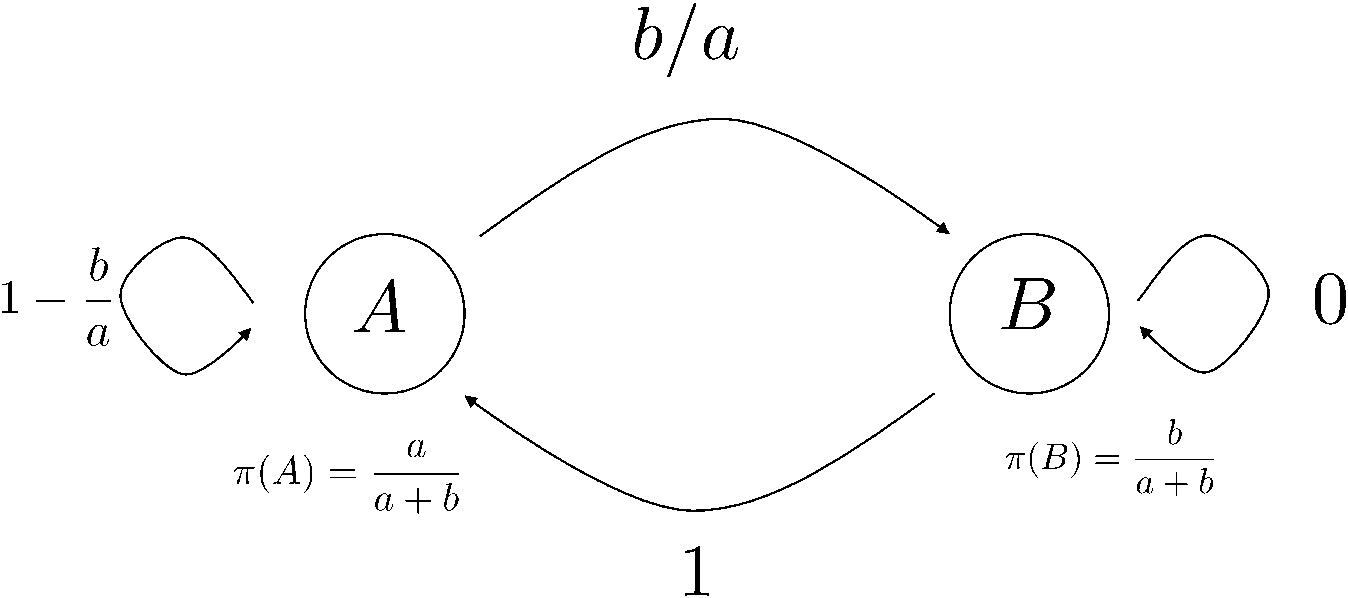
\includegraphics[bb = 0 0 647 287,width=0.5\linewidth]{level2.pdf}
\end{center}
\caption{二準位系におけるMetropolis法のマルコフ遷移図。}
\label{fig_level2}
\end{figure}
\section{二準位系の場合}
状態$A$、$B$の二準位系を考える。それぞれのエネルギーを$E_A$、$E_B$とし、
逆温度を$\beta$とする。ここで、$E_A < E_B$としても一般性を失わない。
\begin{eqnarray}
a &\equiv& \exp(-\beta E_A)\\ 
b &\equiv& \exp(-\beta E_B)
\end{eqnarray}
と略記すると、それぞれの平衡状態での存在確率$\pi(A)$、$\pi(B)$は、
\begin{eqnarray}
\pi(A) &=& \frac{a}{a+b}\\
\pi(B) &=& \frac{b}{a+b}
\end{eqnarray}
と表される。なお、$E_A < E_B$より、$a>b$である。
さて、平衡状態における棄却確率を考える。
平衡状態における棄却確率$R$とは、一ステップ後に現在の状態にとどまる確率、すなわち
\begin{equation}
R \equiv \sum_X^{A,B} \pi(X) P(X \rightarrow X)
\end{equation}
として定義する。ただし$P(X \rightarrow Y)$は状態$X$から状態$Y$への遷移確率とする。
Metroplis法の場合、棄却確率$R_\mathrm{M}$は
\begin{eqnarray}
R_\mathrm{M} &=& \left(1 -\frac{b}{a}\right) \frac{a}{a+b} \\
&=& \frac{a-b}{a+b}
\end{eqnarray}
である(図\ref{fig_level2}参照)。
熱浴法の場合、新しい状態は現在の状態に関係なく、平衡状態での存在確率$\pi$に比例して決まる。
したがって、棄却確率$R_\mathrm{hb}$は
\begin{eqnarray}
R_\mathrm{hb} &=& \pi(A)^2 +\pi(B)^2\\
&=& \frac{a^2+b^2}{(a+b)^2}
\end{eqnarray}
となる。ここで、状態$A$のエネルギー$E_A$を原点に取り直す($E_A=0$とする)。
すると$a=1$となるので、
\begin{eqnarray}
R_\mathrm{M} &=& \frac{1-b}{1+b} \\
R_\mathrm{hb} &=& \frac{1+b^2}{(1+b)^2}
\end{eqnarray}
したがって、
\begin{equation}
R_\mathrm{hb} - R_\mathrm{M} = \frac{2 b^2}{(1+b)^2} >0
\end{equation}
つまり、Metropolis法よりも、熱浴法のほうが常に棄却率が高いことがわかる。
一般に、二準位系においては、詳細釣り合い条件を満たす範囲においては
Metroplis方がもっとも平均棄却率が低いことを証明できる。





\begin{figure}[tb]
\begin{center}
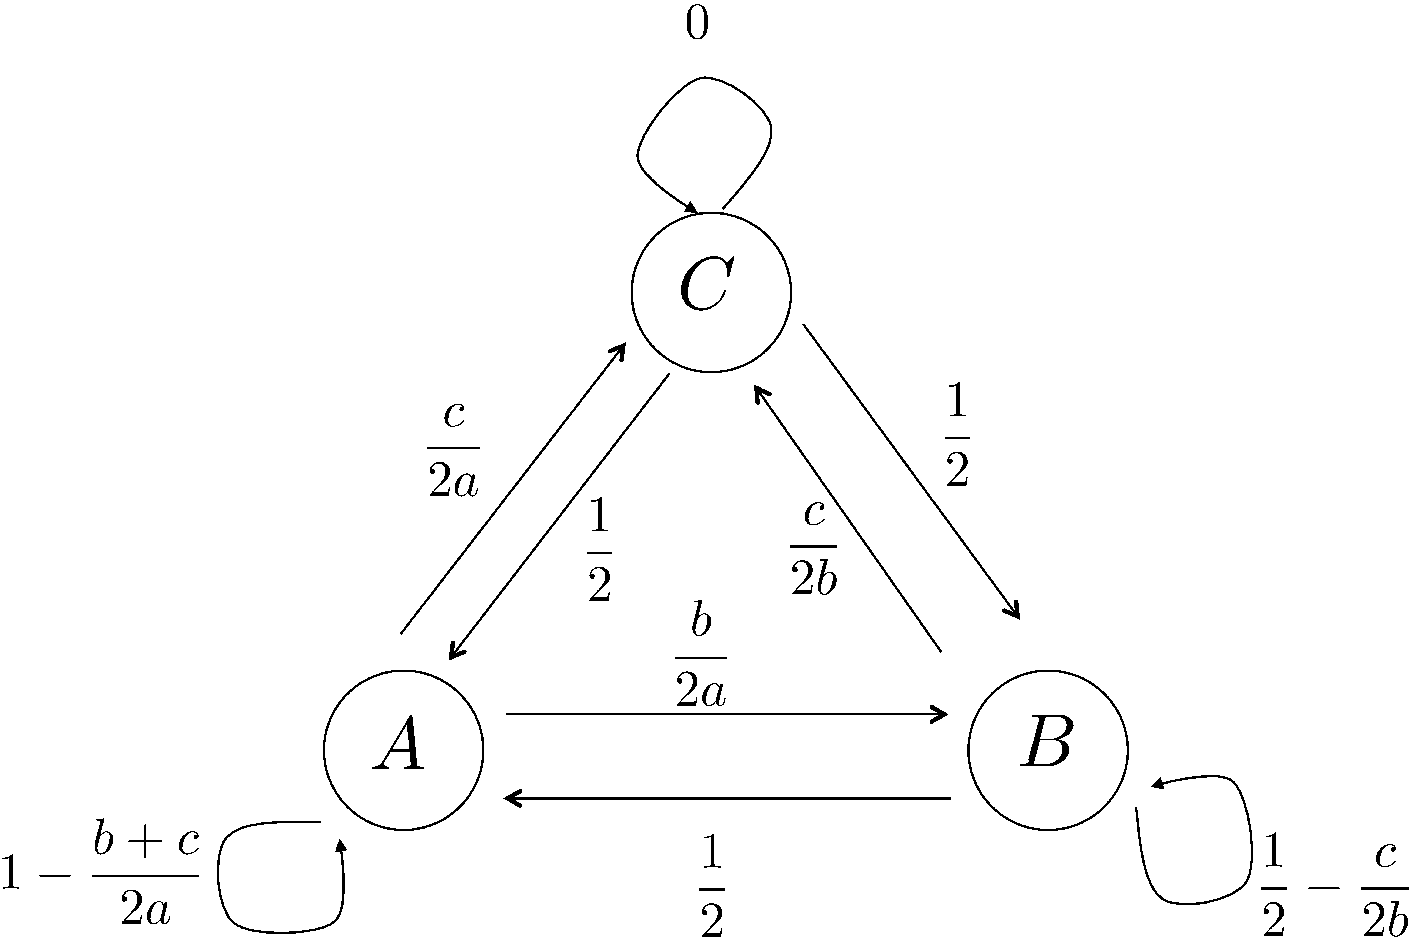
\includegraphics[bb =0 0 678 475,width=0.5\linewidth]{level3.pdf}
\end{center}
\caption{三準位系におけるMetropolis法のマルコフ遷移図。}
\label{fig_level3}
\end{figure}

\section{三準位系の場合}


三準位系でも同様に棄却率を計算してみる。
状態は$A, B, C$とし、$E_A < E_B < E_C$とする。
二準位系と同様に重み$a, b, c$を導入すると。
Metroplis法の場合の棄却確率$R_\mathrm{M}$は
\begin{eqnarray}
R_\mathrm{M} &=& \left(1 -\frac{b+c}{2a} \right) \pi(A)  + \left(\frac{1}{2} - \frac{c}{2b} \right) \pi(B)\\
&=& \frac{a-c}{a+b+c}
\end{eqnarray}
となる((図\ref{fig_level3}参照))。
熱浴法では
\begin{eqnarray}
R_\mathrm{hb} &=& \pi(A)^2 +\pi(B)^2 + \pi(C)^2\\
&=& \frac{a^2+b^2+c^2}{(a+b+c)^2}
\end{eqnarray}
二準位系と同様に状態$A$のエネルギーを原点に取り直し($a=1$)、棄却率の差を計算すると
\begin{equation}
R_\mathrm{hb} - R_\mathrm{M} = \frac{b^2 + (c-1) b + 2 c^2}{(1+b+c)^2}
\end{equation}
この値は、$b$と$c$の値により正にも負にもなる。したがって、熱浴法とMetropolis法のどちらが
棄却率が低いかは条件に依存する(図\ref{fig_graph})。


\begin{figure}[bt]
\begin{center}
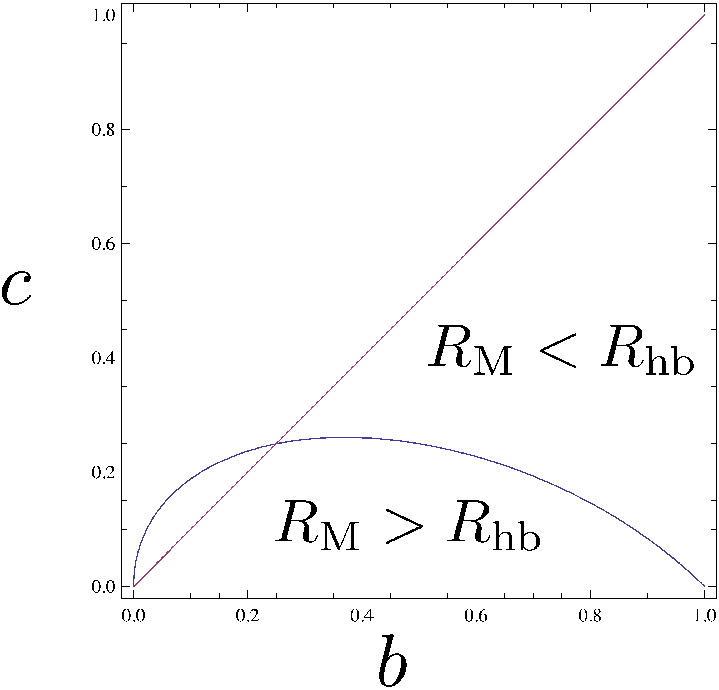
\includegraphics[bb =0 0 345 331,width=0.4\linewidth]{graph2.pdf}
\end{center}
\caption{三準位系における棄却率。$b>c$の領域で、下の方は熱浴法のほうがMetropolis法よりも棄却率が低くなる。}
\label{fig_graph}
\end{figure}

\section{考察}

遷移確率は詳細釣り合い条件だけでは決まらないため、そこに自由度が存在する。
二準位系においては、「平衡状態における棄却率を最小化する」という要請により
Metropolis法が選ばれるが、三準位以上の系においては、熱浴法とMetropolis法の
どちらが棄却率が低いかは条件に依存する。
また、三準位以上の系においては熱浴法、Metropolis法のどちらよりも
棄却率の低い遷移確率の決め方があるのかもしれないし、
実は熱浴法かMetropolis法のどちらかになってしまうのかもしれないが、
面倒なのでまだ計算していない。


\section{Appendix}

一般に$N$状態のMetropolis法の棄却率は
\begin{equation}
R = \frac{1}{N-1}\sum_{k=1}^N (N+1-2k) \pi_k
\end{equation}
で、熱浴法の平均棄却率は
\begin{equation}
R = \sum_{k=1}^N \pi_k^2
\end{equation}
で与えられる。

\end{document}


